\begin{figure}[bt]
    \centering
        \begin{subfigure}{\textwidth}
        \centering
        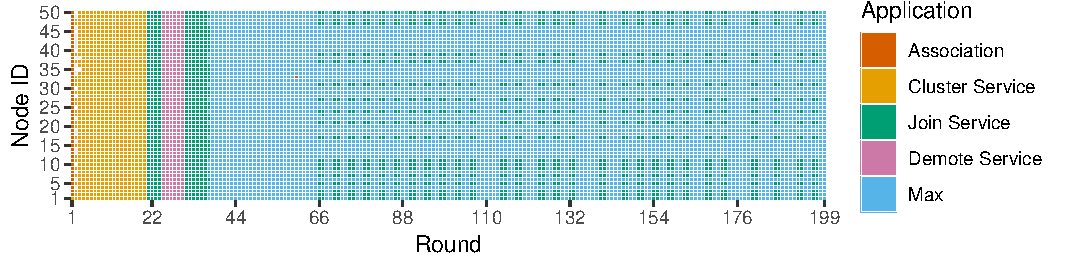
\includegraphics[width=\textwidth, keepaspectratio]{figure/Results/Discussion/applicationmap-50nodes-1000x1000-max-off-run1-bad.pdf}
        \caption{Some nodes are unable to join and therefore frequently schedule the join service resulting in a reliability of $51.2\%$.}
        \label{subfig:application-map-bad-clustering}
    \end{subfigure}
    \hfill
    \begin{subfigure}{\textwidth}
        \centering
        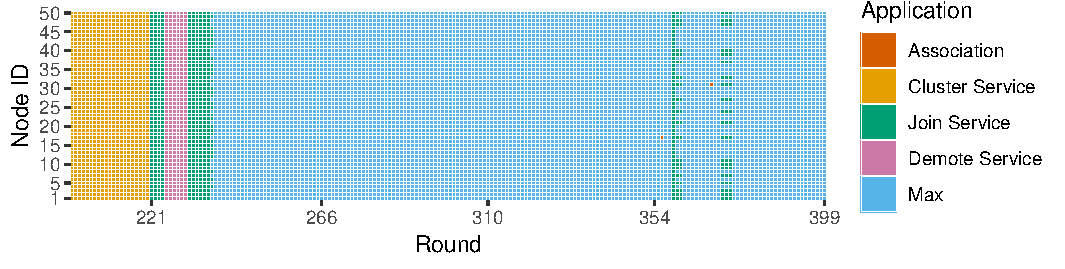
\includegraphics[width=\textwidth, keepaspectratio]{figure/Results/Discussion/applicationmap-50nodes-1000x1000-max-off-run5-good.pdf}
        \caption{A good run with few interruptions due to nodes scheduling the join service resulting in a reliability of $98.6\%$.}
        \label{subfig:application-map-good-clustering}
    \end{subfigure}
    \caption{An example of two application maps for two networks with 50 nodes and an area of 1000x1000 meters.}
    \label{fig:application-map-comparing-good-and-bad-clustering}
\end{figure}